\documentclass[11pt,a4paper]{article}

\usepackage[utf8]{inputenc}
\usepackage[T1]{fontenc}
\usepackage{mathpazo} 
\usepackage[scaled=0.92]{helvet}
\usepackage[margin=1in]{geometry}
\usepackage{graphicx}
\usepackage{amsmath,amssymb,amsfonts}
\usepackage{booktabs}
\usepackage{setspace}
\usepackage{titlesec}
\usepackage{fancyhdr}
\usepackage{tikz}
\usepackage[hidelinks]{hyperref}

\setstretch{1.15}
\setlength{\parindent}{0pt}
\setlength{\parskip}{8pt}

\titleformat{\section}{\normalfont\large\bfseries\sffamily}{\thesection}{1em}{}
\titleformat{\subsection}{\normalfont\normalsize\bfseries\sffamily}{\thesubsection}{1em}{}

\pagestyle{fancy}
\fancyhf{}
\fancyhead[L]{\small\sffamily Apa Itu Variabel? Sebuah Kajian Lintas Disiplin}
\fancyhead[R]{\small\sffamily\thepage}
\renewcommand{\headrulewidth}{0.4pt}

\renewenvironment{abstract}
{\small
	\begin{center}\textbf{\sffamily Abstract}\end{center}
	\begin{quote}}
	{\end{quote}}

\title{\vspace{-1cm}\textbf{\sffamily\LARGE Apa Itu Variabel?\\ Sebuah Kajian Komprehensif Lintas Disiplin Ilmu}}
\author{
	\textbf{Nama Kamu} \\
	\small Program Studi Teknik Rekayasa Perangkat Lunak \\
	\small Politeknik Negeri Batam \\
	\small \texttt{emailkamu@student.polibatam.ac.id}
}
\date{\small\today}

\begin{document}

\maketitle
\thispagestyle{empty}

\begin{abstract}
	Istilah "variabel" (variable) merupakan salah satu konsep paling fundamental yang hadir di berbagai cabang ilmu pengetahuan, mulai dari matematika murni, ilmu komputer, hingga metodologi penelitian sosial. Meskipun terminologinya sama, esensi dan operasionalisasi variabel dapat berbeda secara signifikan antar disiplin ilmu. Makalah ini menyajikan kajian komprehensif mengenai definisi, sejarah, dan aplikasi variabel dari tiga perspektif utama. Dalam matematika, variabel dibahas sebagai simbol abstrak yang merepresentasikan objek atau nilai yang tidak diketahui. Dalam ilmu komputer, variabel dipahami sebagai abstraksi lokasi penyimpanan yang dipasangkan dengan nama simbolik, di mana pada beberapa bahasa modern (seperti Rust) konsep ini lebih tepat disebut sebagai \textit{binding}. Sementara dalam penelitian, variabel dipahami sebagai representasi operasional dari sebuah atribut yang memiliki level pengukuran tertentu. Melalui penelusuran literatur dan visualisasi konseptual, makalah ini bertujuan untuk memberikan pemahaman holistik mengenai bagaimana satu konsep dapat berevolusi dan diadaptasi sesuai dengan kebutuhan spesifik masing-masing bidang keilmuan.
\end{abstract}

\section{Pendahuluan}

Dalam setiap upaya manusia untuk memahami dan memanipulasi dunia, baik itu dunia abstrak dari angka dan logika, dunia digital dari perangkat lunak, maupun dunia nyata dari fenomena sosial, manusia membutuhkan alat untuk merepresentasikan informasi. Alat tersebut dikenal dengan sebutan variabel. Secara etimologis, kata "variabel" berasal dari bahasa Latin \textit{variabilis} yang berarti "dapat berubah" \cite{wikipedia_math}. Namun, seiring dengan perkembangan peradaban dan lahirnya disiplin-disiplin ilmu baru, makna dan peran variabel telah mengalami metamorfosis yang panjang.

Makalah ini membedah konsep variabel dari tiga kacamata yang berbeda. Bagian pertama akan membahas variabel dalam ranah matematika, menelusuri jejak sejarahnya dari peradaban Mesir Kuno hingga notasi modern yang kita kenal saat ini. Bagian kedua akan berfokus pada variabel dalam ilmu komputer, khususnya bahasa pemrograman tingkat tinggi, di mana variabel berfungsi sebagai entitas yang menjembatani logika manusia dengan memori mesin. Bagian ketiga akan mengupas tuntas bagaimana variabel didefinisikan dan dioperasionalisasikan dalam konteks penelitian ilmiah, di mana variabel berfungsi sebagai jembatan antara konsep teoritis dan data empiris.

\section{Variabel dalam Perspektif Matematika}

Dalam matematika, variabel didefinisikan sebagai sebuah simbol, yang biasanya berupa huruf, yang merujuk pada suatu objek matematika yang tidak ditentukan secara spesifik \cite{sobolev}. Penggunaan simbol ini memungkinkan matematikawan untuk merumuskan persamaan dan generalisasi yang berlaku universal, terlepas dari nilai spesifik yang mungkin dimiliki oleh variabel tersebut.

Sejarah penggunaan variabel dalam matematika sangatlah panjang. Jejak paling awal dapat ditelusuri hingga peradaban Mesir Kuno sekitar tahun 1500 SM melalui \textit{Moscow Mathematical Papyrus} dan \textit{Rhind Mathematical Papyrus}. Pada masa itu, masalah-masalah matematika yang melibatkan kuantitas yang tidak diketahui dijelaskan secara retoris, yang dikenal sebagai "Aha problems" \cite{wikipedia_math}. Kuantitas yang tidak diketahui tersebut disebut sebagai \textit{aha} atau "tumpukan".

Memasuki era Yunani Kuno, karya-karya seperti \textit{Elements} karya Euclid (sekitar 300 SM) mendeskripsikan matematika secara geometris. Kemudian, pada abad ke-3 Masehi, Diophantus dari Alexandria memperkenalkan bentuk awal aljabar sinkopasi dalam karyanya yang berjudul \textit{Arithmetica} \cite{boyer}. Diophantus menggunakan simbol khusus untuk merepresentasikan variabel yang tidak diketahui, meskipun ia belum memiliki simbol untuk operasi dan relasi seperti yang kita gunakan sekarang.

Notasi variabel modern yang kita kenal saat ini baru muncul pada akhir abad ke-16 dan awal abad ke-17. François Viète memperkenalkan ide merepresentasikan angka yang diketahui dan tidak diketahui dengan huruf. Konvensi ini kemudian disempurnakan oleh René Descartes pada tahun 1637, yang memperkenalkan kebiasaan menggunakan huruf akhir alfabet seperti \(x\), \(y\), dan \(z\) untuk merepresentasikan variabel (nilai yang tidak diketahui), serta huruf awal alfabet seperti \(a\), \(b\), dan \(c\) untuk merepresentasikan konstanta atau parameter \cite{wikipedia_math}.

Dalam perkembangan selanjutnya, variabel dalam matematika dapat memainkan beberapa peran berbeda. Sebuah variabel dapat berperan sebagai \textit{unknown} (nilai yang harus dicari dalam sebuah persamaan), sebagai \textit{parameter} (nilai yang dianggap tetap selama proses penyelesaian masalah tertentu), atau sebagai \textit{indeterminate} (simbol yang digunakan dalam polinomial atau deret pangkat formal) \cite{wikipedia_math}. Memasuki abad ke-19, Karl Weierstrass memperkenalkan formalisme baru yang mengubah pemahaman intuitif tentang "limit" (di mana variabel dianggap bergerak mendekati suatu nilai) menjadi definisi statis yang ketat. Sejak saat itu, pemahaman modern terhadap variabel matematika bergeser menjadi sekadar simbol yang merepresentasikan objek matematika yang tidak diketahui atau dapat digantikan oleh elemen dari himpunan tertentu \cite{wikipedia_math}.

\section{Variabel dalam Ilmu Komputer}

Berbeda dengan matematika yang memperlakukan variabel sebagai konsep abstrak, ilmu komputer, khususnya dalam bahasa pemrograman tingkat tinggi, mendefinisikan variabel sebagai abstraksi lokasi penyimpanan yang dipasangkan dengan nama simbolik \cite{brookshear, wikipedia_cs}. Penting untuk dicatat bahwa representasi variabel di dalam memori sangat bergantung pada bahasa pemrogramannya. Pada bahasa seperti C atau C++, variabel biasanya merepresentasikan alamat memori spesifik dan membutuhkan kompilator untuk menggantikan nama simbolik dengan alamat tersebut. Namun, pada bahasa dinamis seperti Python atau Ruby, variabel lebih tepat dipandang sebagai nama yang diasosiasikan dengan suatu objek, dan alokasi memorinya ditangani secara transparan oleh \textit{runtime} atau \textit{interpreter} \cite{wikipedia_cs}.

Dalam konteks bahasa pemrograman modern seperti Rust, istilah yang lebih tepat untuk variabel adalah \textit{binding}, yaitu proses mengikat sebuah nama ke sebuah nilai \cite{klabnik}.

\begin{figure}[htbp]
	\centering
	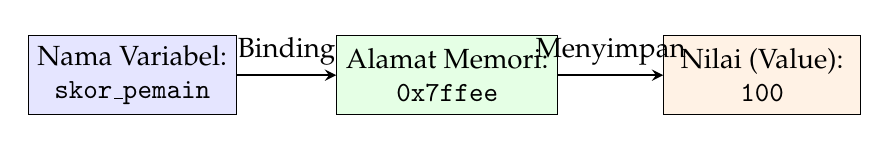
\begin{tikzpicture}[
			box/.style={draw, rectangle, minimum width=2.5cm, minimum height=1cm, align=center},
			arrow/.style={->, >=stealth, thick}
		]
		\node[box, fill=blue!10] (nama) at (0,0) {Nama Variabel:\\ \texttt{skor\_pemain}};
		\node[box, fill=green!10] (alamat) at (4,0) {Alamat Memori:\\ \texttt{0x7ffee}};
		\node[box, fill=orange!10] (nilai) at (8,0) {Nilai (Value):\\ \texttt{100}};

		\draw[arrow] (nama) -- (alamat) node[midway, above] {Binding};
		\draw[arrow] (alamat) -- (nilai) node[midway, above] {Menyimpan};
	\end{tikzpicture}
	\caption{Ilustrasi Konsep \textit{Binding} dan Alokasi Memori pada Variabel Ilmu Komputer.}
	\label{fig:komputer_memori}
\end{figure}

Atribut penting dari sebuah variabel dalam ilmu komputer terbagi menjadi beberapa aspek. Aspek pertama adalah \textit{Scope} (ruang lingkup) dan \textit{Extent} (jangka waktu). \textit{Scope} mendefinisikan di mana teks program variabel dapat diakses, sedangkan \textit{extent} mendefinisikan kapan dalam waktu eksekusi variabel tersebut memiliki nilai yang bermakna. Berdasarkan masa hidupnya, variabel dapat diklasifikasikan menjadi \textit{static variable} (dialokasikan sebelum eksekusi dan tetap ada), \textit{stack-dynamic variable} (dialokasikan saat fungsi dipanggil), \textit{explicit heap-dynamic variable} (dialokasikan secara manual oleh pemrogram), dan \textit{implicit heap-dynamic variable} (dialokasikan otomatis saat nilai diikatkan) \cite{wikipedia_cs}.

Aspek selanjutnya adalah \textit{Typing} (Tipe Data). Dalam bahasa dengan tipe statis (seperti C atau C++), variabel terikat pada tipe data tertentu. Sebaliknya, dalam bahasa dengan tipe dinamis, tipe data melekat pada \textit{nilai} atau objek, bukan pada nama variabelnya; sebuah nama variabel dapat diikat ulang ke objek dengan tipe yang berbeda \cite{wikipedia_cs}. Aspek terakhir adalah fenomena \textit{Aliasing}, yaitu situasi di mana satu lokasi penyimpanan yang sama dapat dirujuk oleh beberapa \textit{identifier} (nama) yang berbeda. Selain itu, parameter formal pada sebuah fungsi juga dikategorikan sebagai variabel yang ruang lingkupnya terbatas pada fungsi tersebut \cite{wikipedia_cs}.

\section{Variabel dan Atribut dalam Metodologi Penelitian}

Dalam dunia penelitian ilmiah, khususnya ilmu sosial dan statistik, pemahaman mengenai variabel bergeser dari sekadar simbol atau lokasi memori menjadi sebuah entitas konseptual yang dapat diukur. Di sini, konsep variabel sangat erat kaitannya dengan "atribut". Menurut Earl R. Babbie dalam bukunya \textit{The Practice of Social Research}, sebuah atribut adalah kualitas atau karakteristik yang melekat pada suatu objek (misalnya, seseorang bisa memiliki atribut "pria", "tinggi", atau "konservatif"). Sementara itu, variabel adalah kumpulan logis dari atribut-atribut tersebut \cite{babbie, wikipedia_research}.

Sebagai contoh, "Jenis Kelamin" adalah sebuah variabel, dan "Pria" serta "Wanita" adalah atribut-atribut yang menyusun variabel tersebut. Variabel dikatakan "bervariasi" karena nilai atau atributnya bisa berbeda-beda antar objek yang diteliti. Perbedaan mendasar antara atribut dan variabel terletak pada tingkat operasionalisasinya. Atribut sering kali bersifat intuitif, sedangkan variabel adalah cara operasional di mana atribut tersebut direpresentasikan untuk keperluan pemrosesan data lebih lanjut \cite{wikipedia_research}.

Nilai dari setiap variabel secara statistik terdistribusi di sepanjang domain variabel tersebut. Domain adalah himpunan dari semua nilai yang mungkin dimiliki oleh sebuah variabel. Dalam metodologi penelitian, level pengukuran variabel secara garis besar dibagi menjadi empat: nominal (kategori tanpa urutan, seperti warna), ordinal (kategori berurutan, seperti tingkat kepuasan), interval (jarak antar nilai bermakna tanpa titik nol absolut, seperti suhu Celsius), dan rasio (memiliki titik nol absolut, seperti berat atau usia) \cite{babbie}.

Sebagai contoh konkret, "Usia" adalah sebuah atribut yang dapat dioperasionalisasikan dengan berbagai cara. Usia dapat didikotomikan menjadi dua nilai saja, yaitu "muda" dan "tua" (variabel biner/nominal). Jika diurutkan, atribut tersebut dapat menjadi variabel ordinal, seperti "muda", "paruh baya", dan "tua". Pada tingkat pengukuran yang paling presisi, usia direpresentasikan sebagai variabel rasio, misalnya 20, 21, atau 22 tahun \cite{wikipedia_research}.

Selain level pengukuran, penelitian juga mengenal peran variabel dalam hubungan sebab-akibat. Variabel independen adalah variabel yang mempengaruhi atau menjadi sebab perubahan variabel lainnya. Variabel dependen adalah variabel yang dipengaruhi atau menjadi akibat. Sementara itu, variabel kontrol adalah variabel yang dianggap konstan atau dikendalikan oleh peneliti agar tidak mengganggu hubungan antara variabel independen dan dependen \cite{babbie}.

\section{Kesimpulan}

Berdasarkan pembahasan di atas, dapat disimpulkan bahwa "variabel" adalah sebuah konsep yang beradaptasi dengan lingkungan disiplin ilmunya. Dalam matematika, variabel adalah simbol murni yang merepresentasikan nilai tak diketahui, yang notasi dan sejarahnya telah berevolusi selama ribuan tahun. Dalam ilmu komputer, variabel adalah abstraksi yang pada saat runtime dipetakan ke lokasi penyimpanan atau nilai tertentu; representasinya di memori bergantung pada bahasa dan implementasinya. Sementara itu, dalam metodologi penelitian, variabel adalah jembatan operasional yang menghubungkan konsep teoritis (atribut) dengan data empiris yang dapat diukur dan dianalisis secara statistik.

Meskipun terdapat perbedaan mendasar dalam cara pandang terhadap variabel, ketiga disiplin ilmu ini memiliki satu kesamaan: variabel digunakan sebagai alat fundamental untuk mengelola kompleksitas informasi, baik itu informasi abstrak dalam bentuk persamaan, informasi biner dalam bentuk data digital, maupun informasi empiris dalam bentuk data penelitian.

\newpage
\section*{Referensi}
\addcontentsline{toc}{section}{Referensi}

\begin{thebibliography}{99}

	\bibitem{babbie}
	Babbie, E. R. (2009). \textit{The Practice of Social Research} (12th ed.). Wadsworth Publishing.

	\bibitem{boyer}
	Boyer, C. B. (1991). \textit{A History of Mathematics}. John Wiley \& Sons.

	\bibitem{brookshear}
	Brookshear, J. G. (2019). \textit{Computer Science: An Overview} (13th ed.). Pearson.

	\bibitem{klabnik}
	Klabnik, S., \& Nichols, C. (2019). \textit{The Rust Programming Language}. No Starch Press.

	\bibitem{sobolev}
	Sobolev, S. K. (n.d.). Individual variable. In \textit{Encyclopedia of Mathematics}. Springer. Diakses dari \url{http://encyclopediaofmath.org/index.php?title=Individual_variable}

	\bibitem{wikipedia_cs}
	Wikipedia Contributors. (2026, October 30). \textit{Variable (high-level programming language)}. Wikipedia, The Free Encyclopedia. Diakses dari \url{https://en.wikipedia.org/wiki/Variable_(high-level_programming_language)}

	\bibitem{wikipedia_math}
	Wikipedia Contributors. (2026, October 3). \textit{Variable (mathematics)}. Wikipedia, The Free Encyclopedia. Diakses dari \url{https://en.wikipedia.org/wiki/Variable_(mathematics)}

	\bibitem{wikipedia_research}
	Wikipedia Contributors. (2026, May 8). \textit{Variable and attribute (research)}. Wikipedia, The Free Encyclopedia. Diakses dari \url{https://en.wikipedia.org/wiki/Variable_and_attribute_(research)}

\end{thebibliography}

\end{document}
